% \chapter{参考文献}

% \begin{figure}[h!]
% \centering
% 		\makebox[0.16\textwidth]{\scriptsize 图像}
% 		\makebox[0.16\textwidth]{\scriptsize 真值}
% 		\makebox[0.16\textwidth]{\scriptsize Grid-5LSTM1}
% 		\makebox[0.16\textwidth]{\scriptsize Grid-5LSTM3}
% 		\makebox[0.16\textwidth]{\scriptsize Grid-5LSTM5} \\
% 		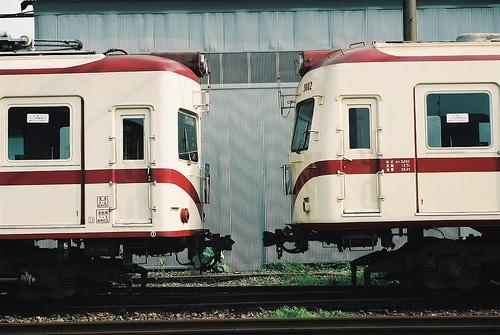
\includegraphics[width=0.16\textwidth]{image/appendix1/2007_000042.jpg}
% 		
\includegraphics[width=0.16\textwidth]{image/appendix1/2007_000042.png}
% 		
\includegraphics[width=0.16\textwidth]{image/appendix1/1/2007_000042.png} 
% 		
\includegraphics[width=0.16\textwidth]{image/appendix1/3/2007_000042.png}
% 		
\includegraphics[width=0.16\textwidth]{image/appendix1/5/2007_000042.png} \\

% 		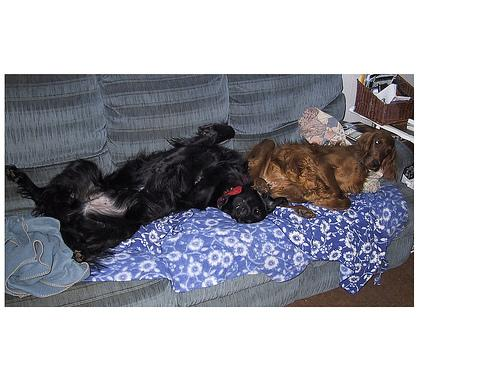
\includegraphics[width=0.16\textwidth]{image/appendix1/2011_003256.jpg}
% 		
\includegraphics[width=0.16\textwidth]{image/appendix1/2011_003256.png}
% 		
\includegraphics[width=0.16\textwidth]{image/appendix1/1/2011_003256.png} 
% 		
\includegraphics[width=0.16\textwidth]{image/appendix1/3/2011_003256.png}
% 		
\includegraphics[width=0.16\textwidth]{image/appendix1/5/2011_003256.png} \\
% 		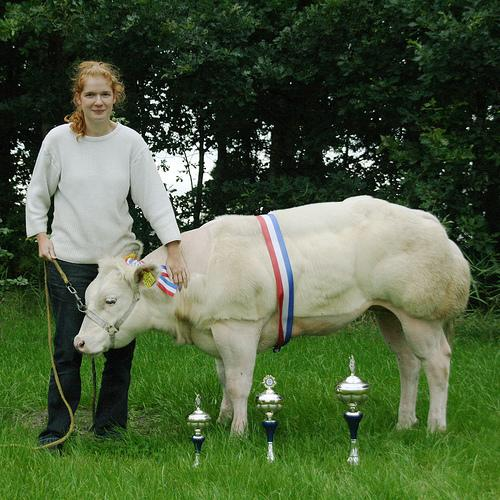
\includegraphics[width=0.16\textwidth]{image/appendix1/2011_001159.jpg}
% 		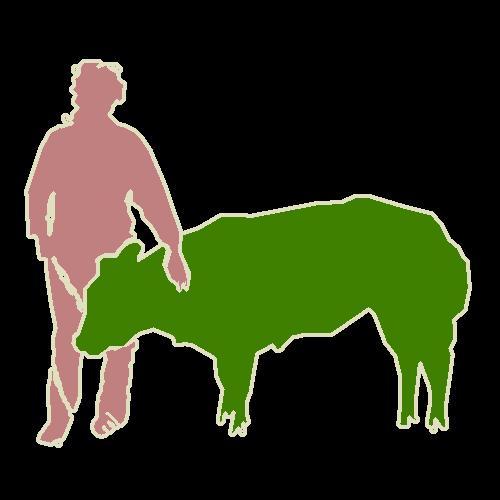
\includegraphics[width=0.16\textwidth]{image/appendix1/2011_001159.png}
% 		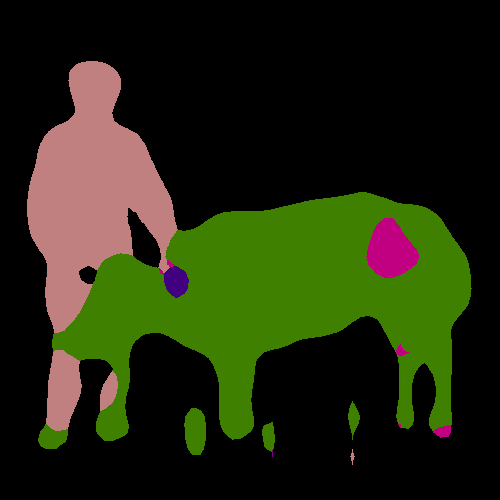
\includegraphics[width=0.16\textwidth]{image/appendix1/1/2011_001159.png} 
% 		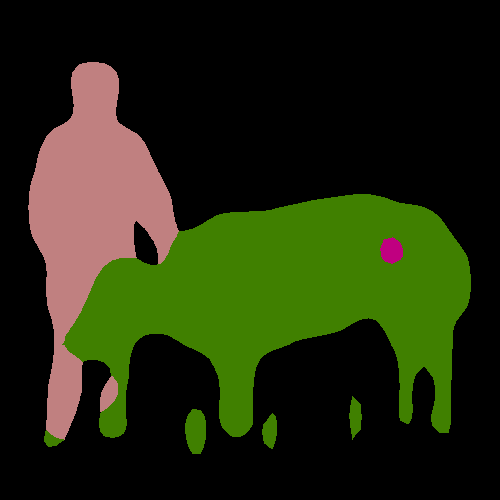
\includegraphics[width=0.16\textwidth]{image/appendix1/3/2011_001159.png}
% 		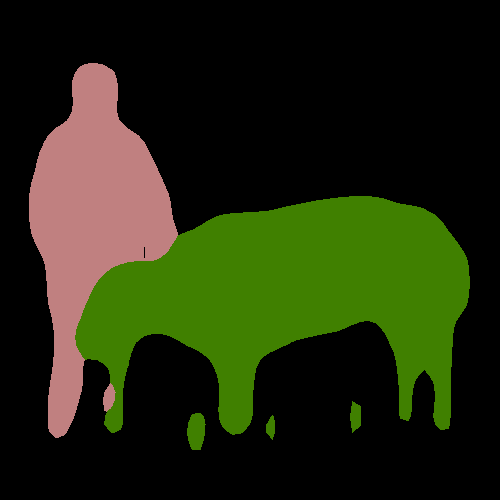
\includegraphics[width=0.16\textwidth]{image/appendix1/5/2011_001159.png} \\
% 		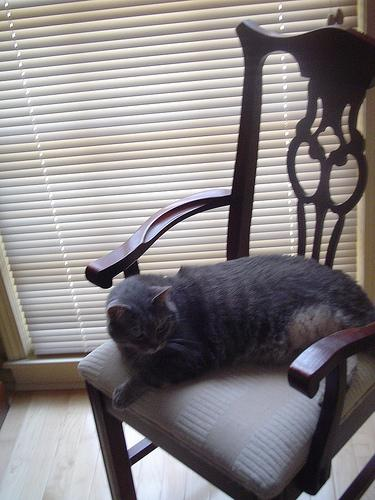
\includegraphics[width=0.16\textwidth]{image/appendix1/2011_000813.jpg}
% 		
\includegraphics[width=0.16\textwidth]{image/appendix1/2011_000813.png}
% 		
\includegraphics[width=0.16\textwidth]{image/appendix1/1/2011_000813.png} 
% 		
\includegraphics[width=0.16\textwidth]{image/appendix1/3/2011_000813.png}
% 		
\includegraphics[width=0.16\textwidth]{image/appendix1/5/2011_000813.png} \\
% 		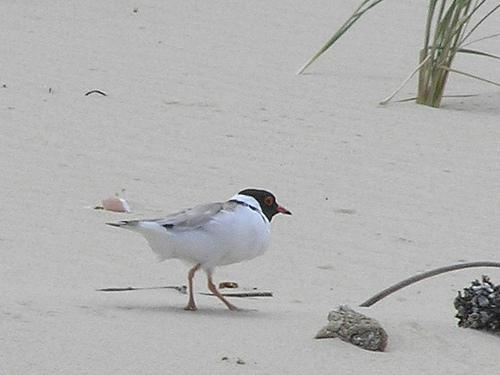
\includegraphics[width=0.16\textwidth]{image/appendix1/2011_003145.jpg}
% 		
\includegraphics[width=0.16\textwidth]{image/appendix1/2011_003145.png}
% 		
\includegraphics[width=0.16\textwidth]{image/appendix1/1/2011_003145.png} 
% 		
\includegraphics[width=0.16\textwidth]{image/appendix1/3/2011_003145.png}
% 		
\includegraphics[width=0.16\textwidth]{image/appendix1/5/2011_003145.png} \\
% 		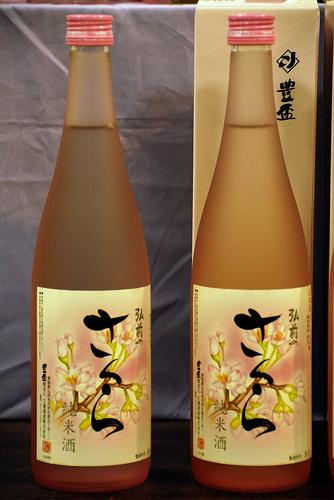
\includegraphics[width=0.16\textwidth]{image/appendix1/2009_004579.jpg}
% 		
\includegraphics[width=0.16\textwidth]{image/appendix1/2009_004579.png}
% 		
\includegraphics[width=0.16\textwidth]{image/appendix1/1/2009_004579.png} 
% 		
\includegraphics[width=0.16\textwidth]{image/appendix1/3/2009_004579.png}
% 		
\includegraphics[width=0.16\textwidth]{image/appendix1/5/2009_004579.png} \\
% \color[rgb]{0.9,0.9,0.9}\bfseries
% \begin{tabular}{*{7}{>{\centering\arraybackslash}p{0.10\textwidth}}}
% 	\hline
% 	\cellcolor[rgb]{0,0,0}  背景&\cellcolor[rgb]{0.5020,0,0} 飞机 &\cellcolor[rgb]{0,0.5020,0} 自行车 &\cellcolor[rgb]{0.5020,0.5020,0} 鸟 &\cellcolor[rgb]{0,0,0.5020} 船   &\cellcolor[rgb]{0.5020,0,0.5020} 瓶子 &\cellcolor[rgb]{0,0.5020,0.5020} 大巴
% 	\\
% 	\hline
% 	\cellcolor[rgb]{0.5020,0.5020,0.5020} 汽车 & \cellcolor[rgb]{0.2510,0,0} 猫 &\cellcolor[rgb]{0.7529,0,0} 椅子 &\cellcolor[rgb]{0.2510,0.5020,0} 牛 &\cellcolor[rgb]{0.7529,0.5020,0} 桌子 &\cellcolor[rgb]{0.2510,0,0.5020} 狗 &\cellcolor[rgb]{0.7529,0,0.5020} 马 \\
% 	\hline
% 	\cellcolor[rgb]{0.2510,0.5020,0.5020} 摩托车 &\cellcolor[rgb]{0.7529,0.5020,0.5020} 人   &\cellcolor[rgb]{0,0.2510,0} 盆栽   &\cellcolor[rgb]{0.5020,0.2510,0} 羊 &\cellcolor[rgb]{0,0.7529,0} 沙发 &\cellcolor[rgb]{0.5020,0.7529,0} 火车 &\cellcolor[rgb]{0,0.2510,0.5020} 电视 \\
% 	\hline
% \end{tabular}

% \caption{一个配有彩色表格的插图}
% \end{figure}

% \endinput
\begin{thebibliography}{123456}
	\bibitem {Gao}Gao C Y,Cui Y B,Heng-TaocL I.A Study of the Application of Basic Path Testing Method[J].Journal of Kaifeng University,2012.
	\bibitem {XU}徐晖,冯永兵,肖传娥,等.基于SQL的数据存储和查询[J].山西电子技术,2001,29(3):15-17
	\bibitem {Yang}杨芙清,梅宏,李克勤.软件复用与软件构件技术[J].电子学报,1999,27(2):68-75.
	\bibitem {Zorro}Ant Design,Ant Design of Angular NG-ZORRO[EB/OL],https://ng.ant.design, 2018-4-20.
	\bibitem {Angular}Angular,Angular中文网[EB/OL],https://www.angular.cn/, 2018-4-20.
	\bibitem {Sequelize}Jonas Zhang,Sequelize Docs 中文版http://docs.sequelizejs.com/, 2018-2-23.
	\bibitem {multer}npm,multer,https://www.npmjs.com/package/multer, 2018-4-20.
	\bibitem {Nodejs}Nodejs,Nodejs中文文档,http://nodejs.cn/, 2018-4-20.
	\bibitem {jm}广发证券互联网金融技术团队.揭秘Angular 2[M].北京:电子工业出版社,2017:20-37.
	\bibitem {Chen}陈文海.软件测试管理工具的研究与实现[D].中国科学院研究生院(软件研究所),2003.
	\bibitem {yuan}袁勤勇.软件工程领域的经典教材——张海藩的《软件工程导论(第5版)》[J].计算机教育,2008,(5):96-97.
	\bibitem {rahayu}Rahayu J A.free,web,hosting,affiliate,unikom,MI,php,mysql[J].
	\bibitem {ng}Ari Lerner; Felipe Coury; Nate Murray; Carlos Taborda.Angular权威教程[M].北京:人民邮电出版社,2017:17-30.
\end{thebibliography}